%\chapter{Collaborative tools}

\renewcommand{\tilde}{\textasciitilde}
\newcommand{\moodle}{Moodle}
\newcommand{\Moodle}{Moodle}

\chapter[\Moodle\ Intro and command line skills]{Introduction to \Moodle\ and command line skills}

\minitoc

\notesurl{intro4}


%\begin{note}
%  This is the fifth, two hour, lab.
%
%  Has change of position (?) of this lab made any difference to how we tell students about first tutorial?  Yes --fixed
%
%  Do we need some breakout boxes in this script?
%
%  \textbf{Steve's wish list}
%  \begin{itemize}
%  \item better navigation---more cd, pushd, popd, mkdir etc
%  \item 
%wildcards (use echo)
%\item 
%fortune | cowsay
%run fortune lots of times to make file
%\item 
%ls m * vs ls m*
%\item 
%revisit handy command line tricks 
%\item where do we introduce dot (as in ./splunge)
%
%  \end{itemize}
%
%
%\end{note}


This is the last of the introductory labs, and is designed to
introduce you to one of the virtual learning environments that's used
in the School, and to give you a chance to practise the command line
skills that you've learned already so that you're ready for when the
regular scheduled labs start. As always, don't rush through
the material, and if you get at all stuck please summon a demonstrator
for help.

\section{Getting started with \moodle}
\label{sec:introduction-moodle}

In the first half of session you'll be introduced to the \moodle\ Virtual Learning Environment (VLE). \moodle\ is an \wikipedia{Open_source}{Open Source} platform designed to support face-to-face teaching by providing an online place to upload resources for course units. It also provides useful tools such as discussion forums and quizzes. We use \moodle\ for several of our course units, which typically have a single `course unit site' within our \moodle\ environment.

%Why is Moodle being used for COMP10120
\moodle\ has several features which make it well suited to supporting this course-unit. These include:
\begin{itemize}
\item It's one useful way of communicating with your tutor and members of your tutor group.
\item It allows us to give each group a wiki which you'll use to collaboratively document your project work.
\item It provides a structure to help organise activities you should be doing on a week-by-week basis.
\end{itemize}

Log in to \moodle\ by pointing your web browser at:
\\

\url{https://moodle.cs.man.ac.uk}
\\

and using your University username and password. 

After successfully logging into \moodle\ for the first time, you'll be presented with a form to complete the details of your \moodle\ profile. Add your first and last names; your email address; the city/town where you live (for most people this will be Manchester); and add a short description of yourself. Select the `Update profile' button to complete your \moodle\ registration. Assuming that worked okay, the next page to appear will be the \moodle\ home page (see  Figure~\ref{figure:moodle-home})

\begin{figure}
\centerline{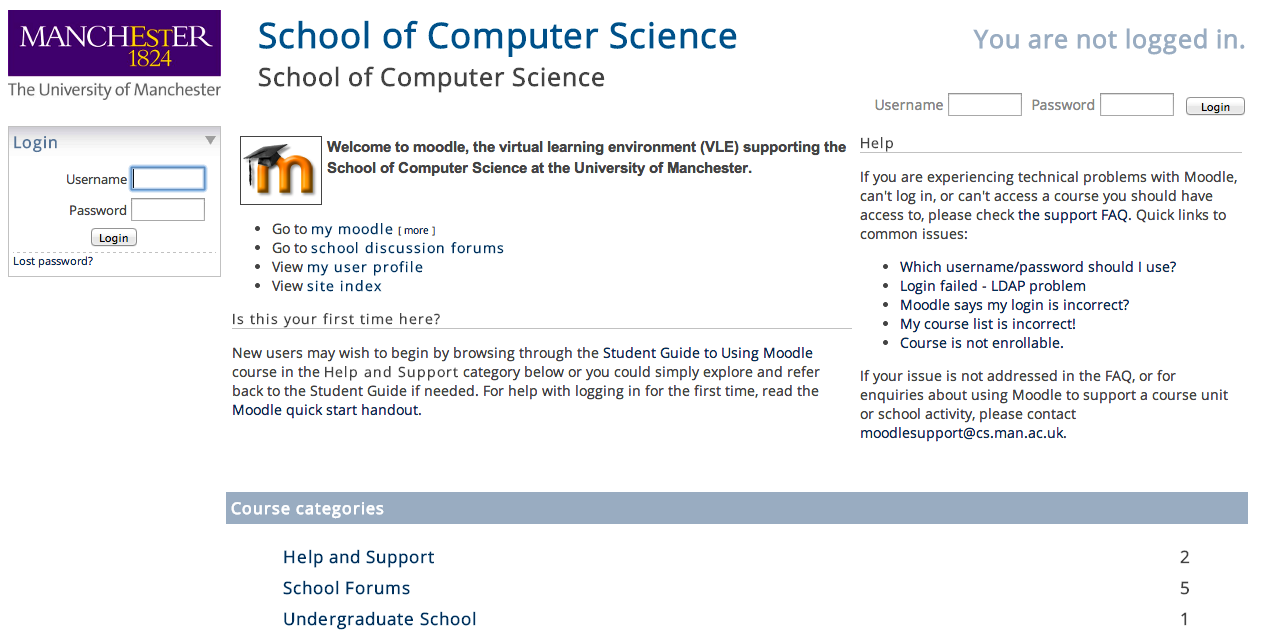
\includegraphics[width=15cm]{images/moodle-home}}
\caption{Moodle Home Page}\label{figure:moodle-home}
\end{figure}

Take a few minutes to browse though the \emph{Getting started with \Moodle} guide which is deliberately located outside the \moodle\ environment so that you can get at it in case you're having problems with \moodle\ itself. You can find it at: \urlnop{octette.cs.man.ac.uk/moodleintro} (see Figure~\ref{figure:moodle-start}).

\begin{figure}
\centerline{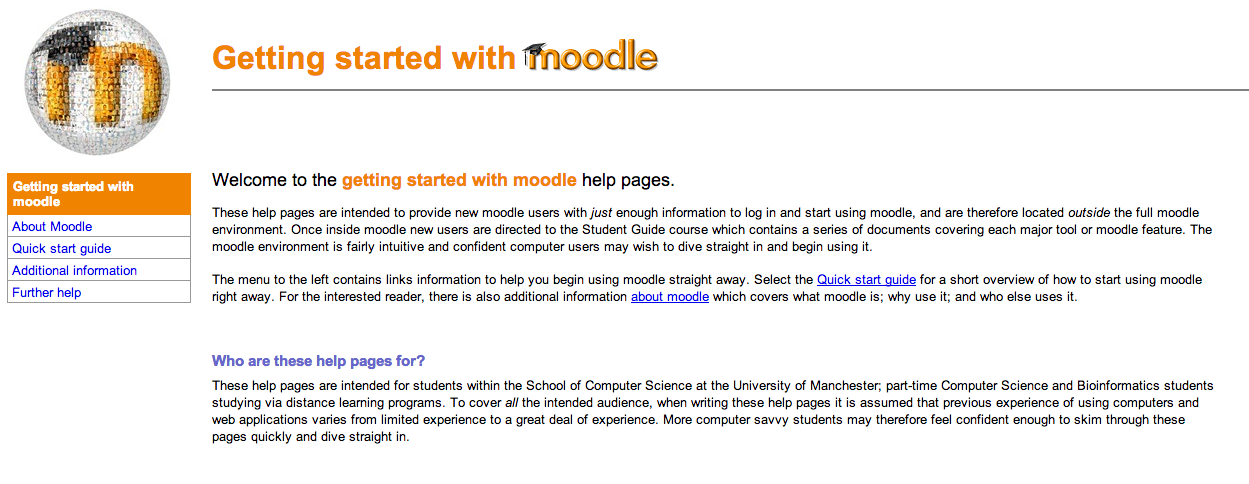
\includegraphics[width=15cm]{images/start-moodle-page}}
\caption{Getting started with Moodle}\label{figure:moodle-start}
\end{figure}

\subsubsection*{Brief overview of the \moodle\ home page}
\label{sec:brief-overv-moodle}


The \moodle\ home page lists several categories in which \moodle\ course unit sites are organised (make sure you scroll down to see them all). \moodle\ course unit sites exist for many, but not all, course units within your degree programme.

You can find links to sites by either locating the link in the appropriate category, for example look in \emph{Undergraduate School/First Year} for COMP10120; or you can enter \emph{COMP10120} into the \emph{Search courses} field at the bottom of the course list and select the course unit title from the search result(s).

Other things to look out for on the front page include the link to your \moodle\ user profile and the link to the \emph{my moodle} feature. We'll come back to these later on.


%Your turn


Make sure you can find the COMP10120 course unit site and are able to access it. To get back to the \emph{\moodle\ home page} you should click on the \moodle\ link in the navigation bar underneath the course unit title at the top of the page. This is always the first element in the link trail. If you navigate further into the course unit site, to return to the \emph{course unit site front page} just click on the COMP10120 link in the navigation bar. This is always the second element in the link trail.

Now locate the course titled \emph{Student Guide to Using Moodle} (in the category \emph{Help and Support}). Have a browse through what help material is provided here. You may wish to revisit this site to learn how to use one of the \moodle\ activities or understand one of \Moodle's features.

\subsection{The COMP10120 course unit site}
\label{sec:comp10120-course-uni}


If you haven't already, navigate to the COMP10120 site and start to look at how the site is structured and what tools have been provided (see Figure~\ref{figure:101-moodle-page}).
Here are some things you should note about the structure of the site:

\begin{figure}
\centerline{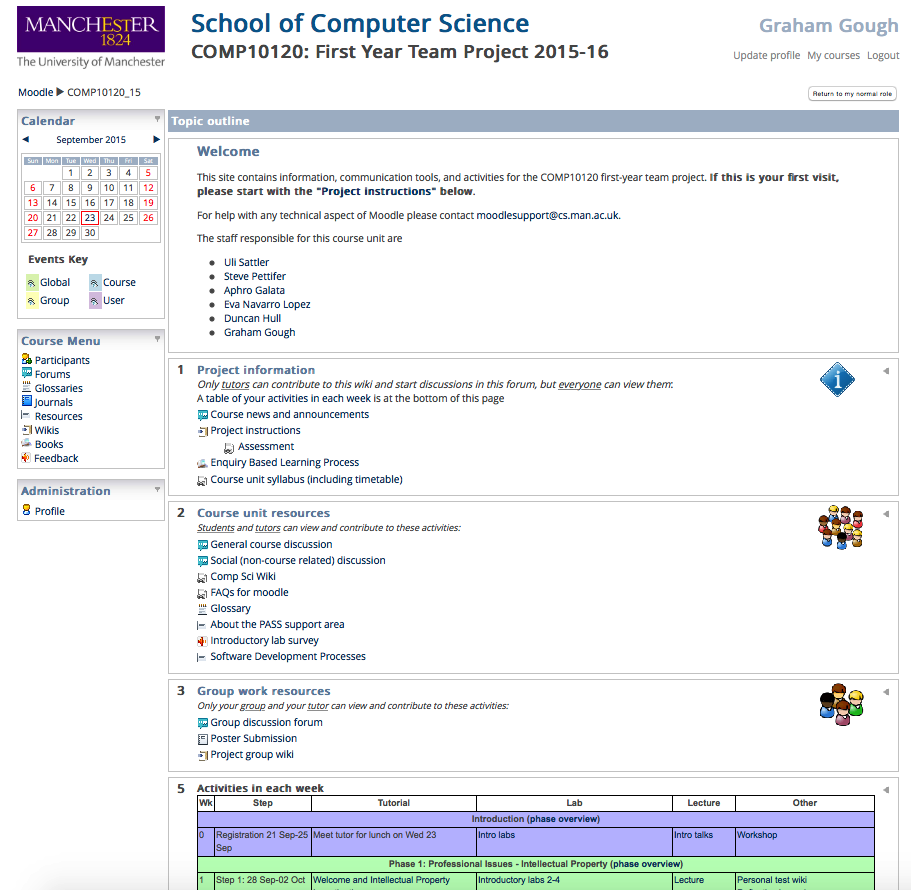
\includegraphics[width=15cm]{images/101-moodle-page}}
\caption{COMP10120 Moodle Home Page}\label{figure:101-moodle-page}
\end{figure}


\begin{itemize}
\item 
All instructions for the course unit are located in the \emph{Project information} area towards the top of the site. Take a look at each of the links in this area. In particular, familiarise yourself with the front page of the \emph{Project instructions} and read at least the \emph{Introduction to the tasks and activities} (and then click through to the \emph{Phases and Tutorials} page to get an idea of the course unit structure).

\item Back on the course unit site, the next section is called \emph{Course unit resources}. If you have a query about the course unit, please use link to the \emph{General Course Discussion Forum}.

\item The next section is called \emph{Group work resources}. This is your tutor group's area and should be used to communicate with members of your team (by using the forum) and to document your work (in the wiki).

\item Finally, the bottom of the course unit site has a table of all your activities for this course-unit. The different phases are colour-coded to help you spot the one you want. The row for each week contains links to information about what you should be doing in that week and tools/resources applicable to the week. (Don't forget to read the \emph{phase overview} first.)

  The \emph{Other}  column includes resources for your personal use, that you are expected to complete over the course of the year. In particular you should note the \emph{reflective journals} for each week of the first semester. You are expected to reflect on the questions detailed inside the journal each week.
\end{itemize}

% The remaining instructions for this lab session can be found
% directly within \moodle\ itself. Click on \emph{Introduction to \Moodle} % in the \emph{Lab} column for \emph{Step 1} in the green (\emph{Phase 1}  section.

\subsection{Lab deliverables}
\label{sec:lab-deliverables}

By the end of this section of the lab session, ensure you have completed the following tasks.

\begin{itemize}
\item 
Posted a welcoming message to your tutor group (see Using forums below).

\item Create your set of practice wiki pages (see Using wikis below).

\item Completed the Individual Learning Profile questionnaire
\end{itemize}

%There are also a number of optional tasks you should aim to complete if you have time during the lab.

\subsection{Using forums}
\label{sec:using-forums}


Most of you will have used discussion forums in some way or another, whether on your favourite social networking site or on some other website. \Moodle's forums aren't too different to any other, however, you should note a few things:

Most forums are configured so that copies of each posting will be emailed to other course unit members. In a group forum, copies are only emailed to other group members; in a course forum copies are emailed to everyone.

In most cases you will have the option to remove your subscription to such emails. Please don't do this, at least not at the moment.

In your user profile you have the option to receive \moodle\ emails as a single daily digest rather than as multiple emails each day; if you're finding you're getting a lot of email from \moodle\ this might be a sensible option to select (but keep it mind that you'll lose some of the immediacy of receiving individual emails). 

You might not be able to post messages in all forums. Some forums (e.g. course announcement forums) will only allow tutors to start new topics of discussion, but will allow students to reply to those topics once started.

%Your turn
Visit your Group discussion forum on the COMP10120 site and click on \emph{Add a new discussion topic}  to begin a new discussion thread. Write a short forum posting to introduce you to your other group members and your tutor. Let them know where you are from, tell them a little bit about yourself.

Note that your discussion posting won't be emailed to the other members of your group until about 30 minutes after you submit the posting. This is to allow time for you to edit it in case you spot a mistake.

If you want to find out more about using discussion forums, look through the \emph{How to use the forums}  help book in the \emph{Student Guide to Using \Moodle} course. There is also a help book called \emph{Using \moodle's HTML editor} which you may also find useful.

\subsection{Using wikis}
\label{sec:using-wikis}


You have almost certainly come across wikis before, and will no doubt have looked things up in \wikipedia{Wikipedia}{Wikipedia}, the world's biggest wiki, many times. Unlike many other online collaboration systems which constrain users in various ways by pre-determining the type of content that can be created (for example sites like Instagram and Flickr are designed for sharing photographs, where as Soundcloud is for sharing audio), and also categorising users as having different types of access (e.g. administrators, moderators, regular users and so forth), the technology behind wikis typically takes a very liberal approach to both users and content. They generally allow any user to make any kind of change to any kind of content, and rely on \textit{social} conventions established by the community to keep things sane. In particular, every edit, deletion and addition to the wiki is stored, providing a complete history of wiki changes. Old versions of pages and be retrieved and compared to new versions of pages. Wikis are typically edited using a simple mark-up syntax where the focus is on content rather than fancy presentation.


As well as creating sites like Wikipedia, wikis are frequently used by software development teams to document their project. The ability to look back to previous versions of documents and the for multiple authors to collaborate on producing the documentation without having to worry too much about `process' is particularly useful in such environments.

During COMP10120 you'll required to document many aspects of your work using a group wiki provided by \Moodle. \Moodle's wiki isn't as powerful as others you may have come across as it is primarily tailored towards teaching, but it does allow you to use \Moodle's standard in-line HTML editor to help you with formatting.

%Your turn
In the \emph{Other} column of the coloured Activities table on the COMP10120 front page you will find a link to a wiki called \emph{Personal test wiki} which is private for you and you only. It is provided to allow you to practise how to use \moodle\ wiki syntax before you start using your shared group wiki. If you have used a wiki before then you may find \Moodle's wiki syntax is slightly different to that which you are used to (in some cases the reverse!).

For this short exercise you will need to read through some of the help documentation hosted inside \moodle. In a new window or tab navigate to \urlnop{moodle.cs.man.ac.uk} again and enter the \emph{Welcome to the Student Guide to Using \Moodle} course in the \moodle\ \emph{Help and Support}  category (you may be asked to 'enrol' on this course, just select 'Yes'). Scroll down to the section about Wikis and select the \emph{How to use the wiki tool} book.

The aim of this short exercise is to create a simple wiki page with two or three wiki links to other pages; incorporate an image; and attach and link to a binary (non-image) file. It is important that you follow this mini-tutorial through to the end as it will ensure you know how to do all the basic tasks needed to help build your own group wiki during the project.

For the purposes of this mini-tutorial you are asked to create a small wiki about yourself.

Start by opening your Personal test wiki. You will be presented with the \moodle\ editor which won't contain any content yet. Enter a title for the page, something like \emph{About Me} will do.

Select the \emph{Save} button. You should now see the first page of your wiki with the content you just added. Now select the \emph{Edit} tab so that you can add more content.

Create a short bullet list containing the items \emph{My hobbies},  \emph{My music}  and \emph{My files}  Save the page again and check the results, then select the Edit tab again. Now turn the three items into wiki links. To do this, just put a single set of square brackets around each of the terms, like this: \emph{[My hobbies]}  \emph{[My music]}  \emph{[My files]}  Save the page again and look at what just happened. If everything worked correctly each term enclosed in square brackets should now look like this: \textbf{term}? (emboldened text followed by a hyperlinked question mark).

Select the question mark symbol on the \emph{My hobbies} term. Note this opens up a new wiki page called \emph{My hobbies} for you to populate with content. Add some text to describe a few things about what you like to do with your time and then select Save.

This is the basic process by which you build up a wiki into a series of linked pages. Note that at the bottom of the page you just created is a list of \emph{Referring links}  This means \emph{a list of pages that link to this one}  Select the link back to the front page.

In the Student Guide to Using \moodle\ course look at the help book on wikis and read the chapter titled \emph{Unique names for pages}  in particular instructions on how to make the link text different from the linked page name. Now go back and change your first wiki page so that the link to the page \emph{My hobbies} contains the link text \emph{My interests} (but still points to My hobbies). Your list should now contain the items \emph{My interests},  \emph{My music}  and \emph{My files} 

Now go back and select the question mark link for the \emph{My music} link and add some content to this page too. You could write about music you love (or music you hate!).

In the last part of this mini-tutorial, you will need to add a small picture to your wiki and a small file. First we need some files to play with. If you have a small picture that you took yourself, great, you own the copyright on it. Create a small text file using any text editor containing any text you like. If you don't have a picture to use and can not source a copyright free image, you will find a link to an example image in the summary text box of the wiki above the first page. There is also a link to a sample text file there too.

In the Student Guide to Using \moodle\ course look at the help book on wikis and read the chapters titled \emph{Attaching binary files} and \emph{Linking to attached files}  From your wiki's front page select the question mark link for the \emph{My files} link to create its page content. Attach your text file to the page from the wiki's Attachments tab as described in the \emph{Attaching binary files} chapter of the help book. Then return to the edit tab and add the following text:

\emph{Wikis allow users to attach files, such as this one here}  

Turn the word \emph{here} into a link to the text file you just uploaded following the instructions in the \emph{Linking to attached files} chapter of the help book.

Carefully read the chapter of the help book titled \emph{Incorporating images}  Now add the following text and add the image you grabbed earlier below the text.

\emph{Wikis also allow users to incorporate images such as this one.} 

Experiment with changing the alignment of the image as described in the help book.

Finally, browse through the remaining documentation in the Wiki help book so that you have an overview of what other information is there and can refer back to it in the future if needed. If you have any questions about how to use the wiki tool, post a message to the General course unit discussion forum.

\subsection{Individual Learning Profile questionnaire}
\label{sec:indiv-learn-prof}

Before the end of the lab session make sure you complete the \emph{Individual Learning Profile questionnaire}. You will find it in the \emph{Other} column of the coloured Activities table on the COMP10120 front page. This activity is to help you to reflect so that you can understand your own basic skills and abilities required for your academic life. It may also be looked at by your personal tutor so the School can be better placed to address your particular needs during your time in the School of Computer Science. This information will only be visible to you, to your tutor and to the course unit organisers.

\subsubsection*{Writing your journal}
\label{sec:writing-your-journal}


One of the aims of this course unit is to encourage you to develop the habit of thinking about the way you are learning and working, and trying to identify ways in which these could be improved. The process of reflection is key to this, but is not something that comes naturally to many of us. In most week slots of the course unit site you will find an instance of the Journal activity. The summary text of each journal contains prompts to aid your reflection that week. The journal is very simple \moodle\ tool which provides you with an editable text area supported by \moodle\ HTML editor. Selecting the \emph{Start or edit my journal entry} button opens your journal. Any entries you put into your journal will be completely private to you and your personal course unit tutor. A limited number of the course unit organisers have access to all students journals, but will respect your privacy and will not be looking at them.

At some time towards the end of this week, start your journal entry for the current week and post your answers the prompts provided.

\subsection{What else is on \moodle?}
\label{sec:what-else-moodle}


As well as course unit sites for many of your course units, there are also a number of open areas within \moodle. Within the \emph{Support Forums} category you will find a number of sites where you can seek help about specific areas within computer science, e.g. the C / C++? Programmer's Forum. The \emph{Student / Staff Groups} category includes a site where you can post up questions or topics of discussion for the Staff Student Consultative Committee. All these open courses are indicated by the guest user icon (a small person icon or a side-on face depending on your chosen \moodle\ theme). Have an explore and see what is there. More open site are likely to be added over the year.

% \subsection*{Playing and personalising}
% \label{sec:play-pers}


% If you have time left in the lab session, spend some time personalising your \moodle\ account. Things you could do include:

% Uploading a small photo or image to represent yourself to your \moodle\ profile.

% %Personalising your my \moodle\ area.

% Take a closer look at the advanced options in your \moodle\ profile and investigate what they do (read up about this in the \moodle\ help course books first).


% % Look ahead on the COMP10120 site to get a feel for what you will be doing over the coming year.

\subsection{Another VLE: Blackboard}
\label{sec:blackboard}

You won't be using it for this course-unit, but for your other course-units you may be using a different Virtual Learning Environment: \textsf{Blackboard}. The usual way to access \textsf{Blackboard} is via the \href{https://my.manchester.ac.uk}{\emph{My Manchester}} page at \urlnop{my.manchester.ac.uk}, and then use the \emph{'My Blackboard'} tab. There is also a plentiful supply of information about how to use Blackboard available online. 

That's all we want to say about Moodle and VLEs. The second part of this lab is about using the command line in Linux.


\section{Reinforcing your command line skills}
\newcommand{\ilinput}[1]{\ttout{#1}}
% \newcommand{\crsname}{COMP10120}
% \newcommand{\Dcrsname}{\fname{/opt/info/courses/COMP10120}}
% \newcommand{\crsnamelc}{comp10120}
\newcommand{\crsname}{INTRO}
\newcommand{\Dcrsname}{\fname{/opt/info/courses/INTRO}}
\newcommand{\crsnamelc}{intro}
\newcommand{\return}{\relax}

This section is designed to help you practise your command line skills in preparation  for next week's start of regular lab activities. You've already used most of these commands in previous labs, but please don't rush through this section since we'll be explaining their behaviour in a bit more detail, and introducing you to some of the extra options they provide, as well as some of the pitfalls that lie in wait for the over-zealous command line user.  

You've probably figured this out already, but it's worth making explicit here: for Unix commands, it's usually the case that no news is good news. So when you run a program from the shell, if you get no response other than your command-prompt back, that almost always means that the command has done what you asked it to (whether you asked it to do what you \textit{wanted} it to do is, of course, an entirely different matter!) Generally speaking, for most simple Unix commands, you can assume that the absence of an error message means that something has worked. And of course, if you get an error or warning message back from a command, it is crucially important that you read it, understand it, and act on it, rather than just ploughing on regardless. If you ignore errors and warnings, bad things happen. This is true in the Unix command world, and probably isn't a bad philosophy for life in general either.

Anyway, back to the exercise and some practice of manipulating files and directories. In previous labs you've already encountered three directories of particular interest:

\begin{itemize}
\item The \concept{root directory} (\ttout{/}) is the top level of the
\concept{file system}.
%??? file system or filesystem ???

\item Your \concept{current working directory} which is the one your are `in'
at the moment (and is shown by the output from \cmdname{pwd}). This can also
be referenced using a single dot (\ttout{.}), as in when starting up Quake Arena using 
\ttout{./ioquake3.arm} in your first Pi lab. 

\item Your \concept{home directory} (\ttout{\tilde}) which is the top level of
your own filestore and where \cmdname{cd} (\concept{change directory}) with no
arguments will take you.  The value of this is also available as
\ttout{\$HOME}, so the following all have the same effect:

\begin{ttoutenv}
\$  cd
\end{ttoutenv}
or
\begin{ttoutenv}
\$  cd \textasciitilde 
\end{ttoutenv}
or
\begin{ttoutenv}
\$  cd \$HOME
\end{ttoutenv}

And no matter what is your current working directory, you can list the files
in your home directory with either of these commands.

\begin{ttoutenv}
\$  ls \textasciitilde
\end{ttoutenv}
or
\begin{ttoutenv}
\$  ls \$HOME 
\end{ttoutenv}

\end{itemize}

You should recall the difference between an \concept{absolute path} (one
that starts with \ttout{/}) and a \concept{relative path} (one that does not
start with \ttout{/} but is instead `found' relatively) by starting in the
current working directory. You've met the `double dot' notation
(\ttout{..}) to mean `go up one level', as in \ttout{ls ..} or perhaps more
often \ttout{cd ..}, or even \ttout{cd ../x/y} and so forth.

Speaking of \cmdname{ls}, you will from time to time need to use its
\ttout{-a} switch argument to ask it to show `hidden' files beginning with a dot,
and/or \ttout{-l} to make it show details about the files it lists.

\subsection{Creating a directory structure}

Use the \cmdname{mkdir} (\concept{make directory}) command
to create some directories. Type:

\begin{ttoutenv}
\$  cd
\$  mkdir \crsname\return
\end{ttoutenv}
%
and check that this directory has indeed appeared using \cmdname{ls}.

It's important that directories we ask you to make for your work have
exactly the names we specify: Unix will let you use any names you
like, but so that demonstrators and staff know where to look for stuff when you get marked, and so that the system you'll be using to submit your work knows what you're submitting, it's very important that you follow these conventions for your lab work. Any files and directories you create for your own purposes outside of lab work can of course be named and organised however you like.

If you made a mistake, e.g. \fname{\crsnamelc} instead of \fname{\crsname},
you can remove the directory \textit{while it is still empty} with the
\cmdname{rmdir} command: e.g.
%
\begin{ttoutenv}
\$  rmdir \crsnamelc\return
\end{ttoutenv}
%
And then try to make it correctly.

%The \cmdname{cd} (\concept{change directory}) command allows you to move around
%the tree by changing your current working directory. Type
%%
%\begin{ttoutenv}
%\$  cd \crsname\return
%\end{ttoutenv}
%%
%to make \crsname{} your working directory. Check that you have changed
%current directory using \cmnd{pwd}{pwd}.
  
Now go into your \ttout{INTRO} directory and let's make some make directories for four imaginary \crsname{} exercises.

\begin{ttoutenv}
\$  mkdir ex1 ex2 ex3 ex4\return
\end{ttoutenv}
%  mkdir ex1 ex2 ex3 ex4 \return
%
%Recall that the \cmdname{cd} command on its own takes you back to your home
%directory, wherever you may be when you invoke it.  Try this out by
%typing
%
%\begin{ttoutenv}
%\$  cd \return
%\end{ttoutenv}
%
%Check that you are now in your home directory.
Now return to your home directory.

Your directory structure should now look something like this:
%\begin{firstonly}
     \begin{center}
       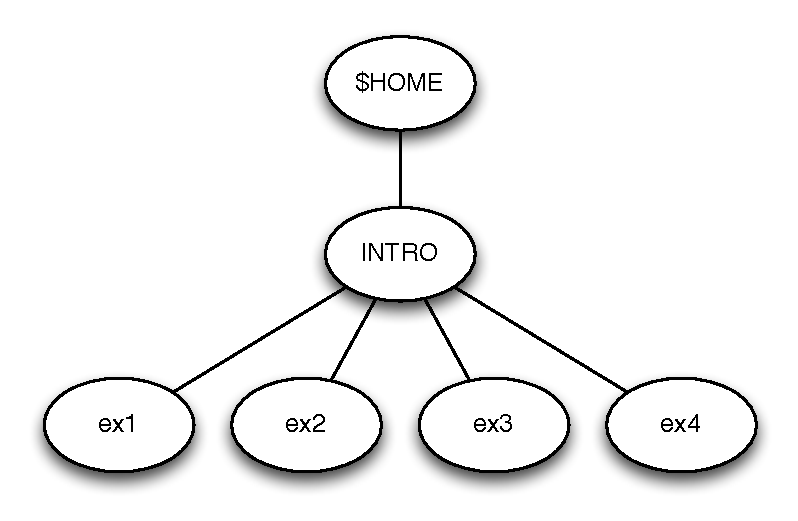
\includegraphics[width=0.6\textwidth]{images/intro-dir-structure}
     \end{center}
%\end{firstonly}

The easiest way to check this is to use 
\cmdname{ls} from your home directory with the \ttout{-R} flag. This shows the whole tree
below your current working directory (as with other commands we've encountered before such as \cmdname{chmod}, here the \ttout{-R} is short for
\wikipedia{Recursion}{recursively}---if you've not looked up what this means yet, now is a good time to do that).

\begin{ttoutenv}
\$ ls -R 
\end{ttoutenv}
%

Next make a directory in your home directory for the
\courseunit{COMP16121} course unit with sub-directories for each of the 10
exercises associated with that course (these aren't imaginary exercises, you'll be starting on them next week). You \emph{must} use the same
convention as above: capital \texttt{COMP16121} and lower case \texttt{ex1} and so on.

You must get your directory structure right before continuing---be extremely careful that you get this right.

%ask a member of the lab staff to check it at this point.

%\begin{note}
%Do we really want them all to ask a demonstrator?
%\end{note}

%Every directory is created with two files already there, called `.'
%and `..'. Of course, you don't see them when you run \cmdname{ls}
%because they start with a dot! Now run the command which will enable
%you to see them in your current directory.
%
%`.' is a reference to the directory itself, and `..'is a reference
%to the directory above it in the tree. This may seem rather bizarre at
%first, but they are in fact extremely useful.  `..', for example,
%enables you to specify a \emph{relative} pathname \emph{up} the tree.

Try the following sequence of \texttt{cd}s, checking where you are by running \cmdname{pwd} after each one, and make sure you understand what is going on: if you're at all unsure about what has happened, please grab a demonstrator to get an explanation---it really will save you a lot of hassle in the long run. 

\begin{ttoutenv}
  cd \return 
  cd \crsname/ex1 \return 
  cd .. \return 
  cd ex2 \return 
  cd ../ex1 \return 
  cd ../../\crsname/ex2 \return 
  cd ../.. \return
\end{ttoutenv}
%

\subsection{Copying, moving, and removing files}

This subsection re-introduces three commands used for copying, moving and
removing files. We'll first describe each command and then you'll get an opportunity  to practise using them.

\subsubsection{Copying files: cp}

\noindent The \cmdname{cp} (copy) command has two forms.

% \begin{note}
%   fix $<$file$>$ [file] notation
% \end{note}

The first general form is
\begin{ttoutenv}
\$  cp [FILENAME] [FILENAME] \return
\end{ttoutenv}

For example

\begin{ttoutenv}
\$  cp file1 file2 \return
\end{ttoutenv}
%
makes a copy of the file \fname{file1} and calls it \fname{file2}.  If
a file called file2 already exists, \emph{the existing \fname{file2} will be  overwritten
with a copy of \fname{file1} and lost without warning}.

The second form is slightly different:
\begin{ttoutenv}
\$  cp [FILENAME(S)] [DIRECTORYNAME]
\end{ttoutenv}
%
For example

\begin{ttoutenv}
\$  cp file1 file2 file3 dirname \return
\end{ttoutenv}

This copies the files \fname{file1}, \fname{file2}, \fname{file3} into
the directory \fname{dirname}, again overwriting any files already
there with the same names.

\subsubsection{Removing/deleting files: rm}

The command \cmdname{rm} (remove) is used to delete files.
\begin{ttoutenv}
\$  rm [FILENAME(S)]
\end{ttoutenv}
%
throws away the specified files. Always take great care when using \cmdname{rm}: unlike putting things in the `trash' or `recycle bin' in a desktop environment, the effects of \cmdname{rm} are \textit{not reversible}, and you don't get any warning before files are \textit{deleted forever}. 


\subsubsection{Moving / renaming files: mv}

The \cmdname{mv} (move) command is similar to \cmdname{cp}, but it just moves
the files rather than makes copies. Again we have the two forms
\begin{ttoutenv}
\$  mv [FILENAME] [FILENAME] \return
\end{ttoutenv}
and
\begin{ttoutenv}
\$  mv [FILENAME(S)] [DIRECTORYNAME] \return
\end{ttoutenv}

The effect is like a copying followed by removing the sources of the copy,
except it is more efficient than that (most of the time).
For example
\begin{ttoutenv}
\$  mv file1 file2 \return
\end{ttoutenv}
is like doing
\begin{ttoutenv}
\$  cp file1 file2 \return
\$  rm file1
\end{ttoutenv}
and
\begin{ttoutenv}
\$  mv file1 file2 file3 dirname \return
\end{ttoutenv}
is like doing
\begin{ttoutenv}
\$  cp file1 file2 file3 dirname \return
\$  rm file1 file2 file3
\end{ttoutenv}


\begin{diversion}{Taking out the trash}
You now know enough about the behaviour of the filesystem to know what's actually going on when you put files in the `recycle bin' or `trash can' in a desktop environment such as you get with OS X, Windows or Gnome. When you `move to trash' in these environments, you're not deleting the file but instead using an equivalent of the \cmdname{mv} command to move the file from its current location into a special directory that represents the trash can. When you tell the graphical environment to `empty trash', you're actually invoking something equivalent to \cmdname{rm}, which actually does delete the file from the filesystem.
\end{diversion}

%\begin{note}
%
%This seems a bit of an odd thing to put in a section about mv. Do we still want to say this?
%
%Before continuing, answer this question and check your answer with a
%member of staff: how do you \emph{rename} a file in Unix? Don't guess---you
%know the answer, unless you have already forgotten from previous labs and you are now going too fast.
%\end{note}


\subsection{Practice makes perfect}
Now for some practice. Go to your home directory by typing:
%
\begin{ttoutenv}
\$  cd \return
\end{ttoutenv}
%
and copy the file called \fname{fortunes} in the \fname{/usr/share/games/fortune}
directory to your current working directory, by typing

\begin{ttoutenv}
\$  cp /usr/share/games/fortune/fortunes \textbf{.}  \return
\end{ttoutenv}
%
Note that the dot (meaning, of course, your current directory) is
essential.  If you now do an \cmdname{ls}, you should see that the
file called \fname{fortunes} has appeared in your directory:

\begin{ttoutenv}
\$  ls \return
\end{ttoutenv}

If no file called \fname{fortunes} has appeared, the following will
probably provide an explanation. If it did appear, read this anyway, just to
check that you understand what you did right.

The \cmdname{cp} command needs at least \emph{two} arguments. In this case, the file
you are copying is \fname{/usr/share/games/fortunes}, and the directory
you are copying it to is `.' (that is, your current working
directory; remember every directory has a reference to itself within
it, called `.') If you missed out the dot, or mis-spelt
\fname{/usr/share/games/fortunes}, or missed out one of the spaces, it
won't have worked. In particular, you may well have got an error message like:
%
%  Usage: cp [-ip] f1 f2; or: cp [-irp] f1 ... fn d2
\begin{ttoutenv}
  cp: missing destination file
  Try `cp --help' for more information.
\end{ttoutenv}
%
or
\begin{ttoutenv}
  cp: /usr/share/games/fortunes/frotunes: No such file or directory
\end{ttoutenv}
%
If you get the first message, it means you used the command with the
wrong number of arguments, and nothing will have happened.
The other is an example of what you might see if you mistype the first
argument. If you do get an error message you need to give the command again,
correctly, to copy the fortunes file across.

\begin{linux}{fortune}
  \label{breakbox:fortune}
  At the moment we're just going to be using the fortunes file as something to copy and move around, so its contents are not important, but it's one of the source files used by the unix \wikipedia{Fortune_(Unix)}{fortune} command, which we will be playing with later.

  \wikipedia{Fortune_(Unix)}{fortune} is a simple program that displays a random message from a database of (supposedly) humorous quotations, such as those that can be found in the US in \wikipedia{Fortune_Cookies}{fortune cookies} (hence the name). It also contains jokes (of a sort!) and bits of poetry.

\end{linux}

You should now have a copy of the file in your home directory.
You'll have to get into the habit of \emph{not} having all your files
in your home directory, otherwise you will quickly have an enormous list
of stuff that will take you ages to find anything in. The use of subdirectories
provides a solution to this problem, which is why you created some
earlier. Moving this file to the `correct' place gives you a chance
to practise the \cmdname{mv} command.

Move the file \fname{fortunes} to your \fname{\crsname/ex4} directory.

% Notice that \fname{\crsname} is \emph{your\/} \crsname{} directory, while
% \fname{\Dcrsname} is (an abbreviation for) \emph{our\/} \crsname{}
% directory, from which you can read things but cannot write to.

Now go to your \fname{\crsname/ex4} directory and check that the file
has appeared there.

To make sure you understand \cmdname{cp}, \cmdname{mv}, and
\cmdname{rm}, go through the following sequence (in your
\fname{\crsname/ex4} directory), checking the result by looking at the
output from \cmdname{ls} at each stage:

\begin{ttoutenv}
\$  cp fortunes fortune1 \return
\$  ls \return
\$  cp fortunes fortune2 \return
\$  ls \return
\$  mv fortune1 fortune3 \return
\$  ls \return
\$  cp fortune3 fortune4 \return
\$  ls \return
\$  rm fortune2 \return
\$  ls \return
\$  rm fortune1 \return
\$  ls \return
\end{ttoutenv}

%\begin{note}
%Should these be fortune1 instead of fortune1? There's really no need to abbreviate names is there? and we may be starting off bad habits when it comes to naming files and variables?
%\end{note}

You'll notice that \ilinput{rm fortune1} behaves differently to \ilinput{rm fortune2}; if you can't figure out why, call a demonstrator for help. 

\subsection{Wild cards}
An asterisk (commonly referred to as \concept{star}) in a filename is a \textbf{wild card} which matches any sequence of
zero or more characters, so for instance, if you were to type (don't
actually do it!)
%
\begin{ttoutenv}
\$  rm *fred*\return
\end{ttoutenv}
%
then all files in the current directory whose names contain the string
`fred' would be removed.

Try the effect of
%
\begin{ttoutenv}
\$  ls fortune*\return
\end{ttoutenv}
%
and
%
\begin{ttoutenv}
\$  ls *tun*\return
\end{ttoutenv}

Now try
%
\begin{ttoutenv}
\$  echo *tun*\return
\end{ttoutenv}
%
Our previous use of \ttout{*} has always been in conjunction with \cmnd{ls}{ls} which might have led you to think that the wild card was being expanded by \cmnd{ls}{ls}. In fact the expansion is done by the \emph{shell}, \cmnd{bash}{bash}, which means that the effect is true for anything you type on the command line. Wildcards are a very powerful and useful feature of the command line, and as with anything powerful and useful can be used or mis-used, so its important that you know what you're doing with them.

One place where you have take care with wild cards is provided by the dotfiles---these are files
whose names begin with a dot (\ttout{.}), and the asterisk will not match a
\ttout{.} at the start of a file name. To see what this means try the
following
\begin{ttoutenv}
\$  cd \return
\$  ls *bash* \return
\end{ttoutenv}
%
and
%
\begin{ttoutenv}
\$  ls .*bash*\return
\end{ttoutenv}
and see the different output.

\subsection{Quotas}
The command

\begin{ttoutenv}
\$  quota\return
\end{ttoutenv}

shows you what your file store quota is, and how much of it you are
actually using. This is only of academic interest now, but may become
very important later in the year! You may find that you are unable to
save files if you use more than your quota of
file store. It is important that, if this happens, you do something
about it immediately.
 
\subsection{Putting commands together} 
\subsubsection{Redirection}  
Before you forget that you're in your home directory, change back to
your \crsname/ex4 directory.

One of the simplest (and most useful) of Unix commands is
\cmdname{cat}. This command has many uses, one of which is to
con\textbf{cat}enate a list of files given as arguments and display
their contents on the screen. For example
\begin{ttoutenv}
\$  cat file1 file2 file3 \return
\end{ttoutenv}
would display the contents of the three files \fname{file1},
\fname{file2} and \fname{file3}.
The output from \cmdname{cat} goes to what is known as the
\textbf{standard output} (in this case the screen).

If you type  
\begin{ttoutenv}
\$  cat \return
\end{ttoutenv}
nothing will happen because you haven't given a file to \cmdname{cat}.
When run like this, it takes its data from the \textbf{standard input}---which in this case is the keyboard---and copies it to the standard
output. Anything that you now type will be taken as input by
\cmdname{cat}, and will be output when each line of the input is
complete. In Unix, end of input is signalled by \ctrl{d}.
(Recall that typing \ctrl{d} in your login shell will log you
out---you have told the shell to expect no more input). So, after
typing \cmdname{cat} above, if you type:
\begin{ttoutenv}
The cat
sat
on the
mat
\end{ttoutenv}


and then press \ctrl{d} you will see the input replicated on the output (interleaved line by line with the input). The first copy is the `echo' of what you typed as
you typed it, the second copy is output from \cmdname{cat}. This may
not seem very useful, and you wouldn't actually use it just like that,
%(An example where you really would have cat do just this is a bit too
%complicated to show here!) 
%We've merely asked you to do that to
but it illustrates the point that \cmdname{cat} takes its input and copies it
to its output. Using this basic idea we can do various things to
change where the input comes from and where the output goes.

\begin{ttoutenv}
\$  cat > fred1
\end{ttoutenv}
will cause the standard output to be directed to the file \fname{fred1}
in the working directory (the input still comes from the keyboard and
will need a \ilinput{<Ctrl>d} to terminate it. Try creating a file
\fname{fred1} using this technique, and then check its contents.

\begin{ttoutenv}
\$  cat < fred1 
\end{ttoutenv}
will take the standard input from the file \fname{fred1}
in the working directory and make it appear on the screen. This has
exactly the same effect as 
\begin{ttoutenv}
\$  cat fred1 
\end{ttoutenv}

You can, of course, use $<$ and $>$ together, as in
\begin{ttoutenv}
\$  cat < fred1 > fred2
\end{ttoutenv}
which will copy the contents of the first file to the second. Try this and
check the results.

We can, of course, do this type of redirection with other
commands. For example, if we want to save the result of listing a
directory's contents into a file we just type something like
\begin{ttoutenv}
\$  ls -l > fred1
\end{ttoutenv}
(this overwrites the previous contents of \fname{fred1} without
warning, so be careful of this kind of use).

% One of the other things that \cmdname{cat} can do is to put line
% numbers on its output. It does this if you use the \ilinput{-n}
% flag. Try
% \begin{ttoutenv}
% \$  cat -n fred1
% \end{ttoutenv}


% Now suppose, for the sake of argument, we wanted to have a listing of the
% names of the
% files in the current directory, with each line numbered, and the result
% saved in a file \cmdname{fred3}. You have just been given all the
% information you need to do this---so, how would you do it? Do it now.

% Unless you've met Unix before, you probably did something like this
% \begin{ttoutenv}
% \$  ls > tmpfile 
% \$  cat -n tmpfile > fred3
% \end{ttoutenv}
% Or if you didn't then try it now and examine the contents of
% \fname{fred3}. The file \fname{tmpfile} can now be thrown away using
% \ilinput{rm tmpfile}.

% It's a shame we had to use an extra, temporary, file. Could we avoid
% having to? Why do you think the following would not work?
% \begin{ttoutenv}
% \$  ls > fred3 
% cat -n fred3 > fred3
% \end{ttoutenv}

% A better way of doing the task, which avoids the use of a temporary file
% is by use of a powerful Unix feature called the \textbf{pipe}. We just type
% \begin{ttoutenv}
% \$  ls | cat -n > fred3
% \end{ttoutenv}

In the previous Intro lab session we met the idea of a \concept{pipe}, using the \verb+|+ symbol to connect the \concept{standard
output} of one command is to be \concept{piped} to the
\concept{standard input} of a second.

We can construct another (admittedly rather artificial) pipeline example using
just \cmdname{cat}:

\begin{ttoutenv}
\$  cat < fred1 | cat > fred2
\end{ttoutenv}

The first \cmdname{cat} takes its input from the file
\fname{fred1} and sends its output into the pipe. The second
\cmdname{cat} takes its input from the pipe (i.e. the output from the
first \cmdname{cat}) and sends its output to the file \fname{fred2}. (How many
other ways can you think of to do this?)  This isn't a very sensible
thing to do, but it does illustrate the principle of piping, and more realistic examples
will appear in the exercises.

Standard output sent to the screen may come so fast that it
disappears off the top before you have had a chance to read it.
There is a simple way around this problem by piping the output into the command \cmdname{less}
  which arranges to stop after each pageful (or screenful, or window-ful) of output. For example,
  \begin{ttoutenv}
  ls -la | less
  \end{ttoutenv}
  would be a wise precaution if the current working directory held
  more than a screenful of entries. When \cmdname{less} has shown you the
  first screenful, press the space bar to see the next screenful,
  or \ttout{return} to see just the next line.

  %\item 
%   Without foresight, the output will rush past you at a great rate
%   of knots. Press \ctrl{s} to stop it dead in its tracks
%   (and \ctrl{q} to set it off again).
%   In practice this isn't much use nowadays---in most cases the computer is
%   just too fast for the Human to press the keys at the right time.
% \end{itemize}

Now would be a good time to remove all those junk files like \fname{fred1} etc.

Before we leave the subject of pipes we meet two of the less obviously
useful Unix commands, \cmdname{fortune} and \ttout{cowsay}. We met
\cmdname{fortune} briefly in Breakbox~\ref{breakbox:fortune}, try
running it a few times now. (Hope you didn't type the command more
than once. If you did, think how that could have been avoided.)

Now try running the command \cmdname{cowsay}. Nothing happens, because
the cow is waiting for you to tell it what to say. Type anything you
like and then \ctrl{d} to denote the end of input. The cow should then
utter your words: 

\begin{verbatim}
 _____________ 
< Hello World >
 ------------- 
        \   ^__^
         \  (oo)\_______
            (__)\       )\/\
                ||----w |
                ||     ||
\end{verbatim}


Now try putting \cmdname{fortune} and \cmdname{cowsay} together to get
the cow to `speak' the fortunes. Utterly useless but it illustrates
the use of pipes.

\subsection{Making your own commands}
\label{sec:making-your-own}

Pretty much anything that you can type at the command line can also be stored in a file to create a simple program called a \concept{shell script}, so if you find yourself frequently connecting together simple commands to perform a particular task, you might find it useful to create a script for use in future, rather than retyping everything each time. If you recall back to Section \ref{section:pipesandredirects} we made a simple command called \texttt{mankyweather} using an \concept{alias}. Aliases are fine for things that you can express in a single line of text, but clumsy for more complex combinations of commands; a shell script instead allows you to use as many lines as you like.

\begin{diversion}{Scripting versus Programming}
You may be wondering what the difference is between a `script' and a `program', or between the idea of `scripting languages' or `programming languages'. It's quite difficult to pin down exact meanings for these, since their use has shifted over time and different people use the terms to mean subtly different things. Scripting languages and programming languages both allow people to create sequences of instructions for a computer to execute. Generally speaking when people refer to scripts or scripting languages the are referring to mechanisms for automating tasks rather than for performing complex computations. So if you wrote something that once a month deleted any files that ended with \fname{.bak} from your filestore, you would probably use a scripting language, and most likely think of it as a script. If you were to write the next 3D blockbuster console game to outsell Grand Theft Auto V, you'd probably use a programming language and think of it as a program. At the extreme ends of the spectrum, the distinction is quite clear; in the middle it gets a bit muddy.
\end{diversion}


Use an editor to create a \concept{shell script} in the file
\ttout{\tilde/bin/wisecow}. Make a directory in your home directory called \fname{bin} using the command:

\begin{ttoutenv}
\$ mkdir \tilde/bin
\end{ttoutenv}

and in that directory create a file called \texttt{wisecow}. You're welcome to use whatever text edito you like for this, but you might find that for short edits like this you're better off using something like \cmdname{nano} rather one of the more heavyweight graphical editors. 

Put the following text into the file:

\begin{ttoutenv}
#!/bin/bash

fortune | cowsay
\end{ttoutenv}

The first line tells the operating system to use the program \ttout{/bin/bash}
when this script is run, i.e. it will start \cmdname{bash} with an argument
telling it to get its commands from this file and execute them pretty much as
though they had been typed into bash in the usual way.

Now try to run your new program:

\begin{ttoutenv}
\$  \tilde/bin/wisecow
\end{ttoutenv}

Oops, that won't have worked! Before the operating system will believe us
that this really is a thing that we can run, we need to give the file \concept{execute
permission}. Use \cmdname{ls} to see what permissions the file has at the
moment. To make it \concept{executable} we use \cmdname{chmod} as follows.

\begin{ttoutenv}
\$  chmod +x \tilde/bin/wisecow
\end{ttoutenv}

Now check its the permission again. If all is okay, you should be able to run
this time with

\begin{ttoutenv}
\$  \tilde/bin/wisecow
\end{ttoutenv}

and your wise cow should have spoken.

Now here is the really cool bit: in an earlier lab you met the idea of
\ttout{\$PATH}---the list of all places where the operating system will
search when you type a command without specifying its full pathname. See the
value of this now:

\begin{ttoutenv}
\$  echo \$PATH
\end{ttoutenv}

Notice one of the directories listed is your very own \ttout{\tilde/bin} directory: this
is where you can put \emph{your own} commands.

So, now type just

\begin{ttoutenv}
\$ wisecow
\end{ttoutenv}

and bask in the wisdom of your newly created cow guru. 

\subsection{Printing text files: lpr}

The command \cmdname{lpr} can be used to send files to a printer. In its
simplest form, you simply run:
%
\begin{ttoutenv}
\$  lpr file1 file2
\end{ttoutenv}
%
to print the given files. The printing service we use is the University \concept{Pull printing} service, which allows you to collect your printing at \emph{any} University pull printer. This is described in more detail at 

{\small
\url{http://www.itservices.manchester.ac.uk/students/printing/}
}

You could use \cmdname{lpr} now to print out the \fname{fortunes}
file, but that file is quite big and we don't want to waste a lot of
paper. So please don't! However, it would be nice to practise using
\cmdname{lpr}. So instead print out just the first 50 lines of
it. Look at the man page for \cmdname{lpr} and discover what it does
if no file names are given. Now look at the man page for the command
\cmdname{head} and figure out how to make it output the first 50 lines
of the file \fname{fortunes}.  Experiment with this to make the 50
lines appear on your screen.
% From what you
% have already learnt, you should know how to check there are exactly 50 lines
% using the counting option of \cmdname{cat}.
Now send the 50 lines to the
printer---without using a temporary file. Go and collect your print output
from a nearby printer (there are printers in SSO, G23, and other places).
%
% head -50 fortunes | lpr

\cmdname{lpr} is a basic printing tool for printing text (and it is also
clever enough to print most types of images nowadays). A more sophisticated
printing program is \cmdname{a2ps}. This produces a nicer output, and it
can recognise different types of text file---including program
source code files---and present the various keywords of the programming
language and the program identifiers in different fonts to help with
readability.

Look at the man page for \cmdname{a2ps} and use \cmdname{a2ps} to print the file
\\

\fname{\Dcrsname/SimpleJavaProgram.java} 
\\

When you collect
this print output you will see that \cmdname{a2ps} has formatted it nicely. This is a
good way to obtain printouts of your own work, should you wish to.

All students have a printing account which is used to `pay' for their printing. The School has pre-credited your account with enough credit for you to print all the material needed for your courses (with some to spare) without having to pay for anything. For administrative reasons, your initial credit will be \pounds4, and this will be topped-up during the year. The first top-up is likely to occur during Reading Week.

The printing allowance we give you means that you will be able to to print 500 sides during the year if you use the double-sided A4 mono option (at 8p per page). Note: the allowance would only cover 400 sides if you use the A4 single-sided option, at 5p per page, so clearly printing double-sided is your better option.

\subsection{Time for a checkup}
\label{sec:time-checkup}

\begin{roadblock}{Check your setup}
Now it's time to check that your CS account's environment is set up properly. In the earlier
introductory labs we got you to make various changes to the configuration files that determine how your account behaves (the so-called `dotfiles').


From a terminal, run the command

\begin{ttoutenv}
/opt/teaching/bin/check-my-setup
  \end{ttoutenv}


If you skipped any of the steps in the intro labs, or didn't quite get things right, then this script will help you detect any configuration issues that might bite you later, and will help you fix any problems it finds (if you're curious about the script works, use less to check out its contents).


If you don't understand what the script is telling you to do, please do take this opportunity to find a demonstrator to explain things.

Once you've fixed any problems that the script has identified, please re-run the script to check everything is now okay, and then repeat this process until the script reports that everything is `good'.
  
\end{roadblock}

\subsection{Exercises}

Here are a number of exercises to experiment with. Use \cmdname{man}
to find full details of the relevant commands you need to use. When you
have your answers, email them to you personal tutor. Just send a
single email with everything in. If you can't complete all the
exercises, no problem, just send what you've done.

%
\begin{enumerate}
%
%\item Select \fname{File Manager} from \fname{Programs} from the
%  workspace menu and explore your filestore visually. Double clicking
%  with the left mouse button on an icon opens a file or directory.
%
\item As you know, \ilinput{ls -l} gives you extra information
 about files. Skim through the man page for \cmdname{ls} to see what
 it means. Check the ownership and permissions of your
 own files. For more
 about ownership and permissions, look at the manual pages for the
 \ttout{chown} and \cmdname{chmod} commands.

 \textbf{Question: Why don't you own `..'  in your home directory?}

%
\item Look at the \cmdname{man} entry for  \cmdname{rm} and find out
  what would happen if you did \cmdname{cd} and then  
  \ilinput{rm  -rf * }\\ 
  \textbf{WARNING! DO NOT ACTUALLY TRY THIS!}  We once had a system administrator who, after
  logging in as the \concept{superuser} (that's a special user called
  \concept{root} that has the permission to do \emph{anything}), typed
  the above command by accident. What do you think happened? (Hint: on
  many Unix systems, the superuser's home directory is /).

\textbf{Question: What would it do in your home directory? What would it do if the
  superuser made this error?}

\item Another useful command is \cmdname{grep}, which displays all
  lines of a file containing a particular string (in fact, the
  string can be a pattern with wild-cards and various other things in).
  The form for a simple use of \cmdname{grep} is
\begin{ttoutenv}
  grep [PATTERN] [FILENAME(S)]
\end{ttoutenv}
%
This will result in a display of all the lines in the files which
contain the given pattern.

A useful file to use for experiments with \cmdname{grep} is
\fname{/usr/share/dict/words}, which is a spelling dictionary. Try to
find all words 
in the dictionary which contain the string `red'.

  \textbf{Question: what was the command you used to do this? (Please don't email your
  tutor the \emph{results} from the command!)}

\item 
  Use a suitable pipeline to find out how many
  words in the dictionary contain the string `red' but not the
  string `fred'.  (Hint: The answer to the previous question gives all
  the words containing `red', look at the manual page for
  \cmdname{grep} to find out how to exclude those words containing
  `fred'. The \cmdname{wc} (short for `word count') program counts words
  (amongst other things). Use pipes to put them all together.)

  \textbf{Question: what was the command you used to do this? How many words did you find?}

% \item Investigate the \cmdname{ps} command, which tells you about the
%   processes (running programs) on your workstation, how much swap
%   space they are using etc..
% \item (Harder) Wander around the top of the directory tree, from /,
%   and try to understand what you find there.
\end{enumerate}

You have now finished the lab, but we encourage you to try the exercises
contained in the file \fname{\Dcrsname/extras}. Don't worry if you find them
tricky---they are.

\subsection{The end of the beginning}

That's it! You've now reached the end of the introductory labs.  

What follows next week in your various courses are labs and coursework
that will actually form part of your assessment, and ultimately, your
Degree.

If you're new to Unix/Linux it's a good idea to spend a bit of time
reflecting on and re-reading through what we've already done in order
to ready yourself. Make sure you feel comfortable with the concepts
we've presented. If something seems a little weird, or hard to follow,
spend a bit of time and go over that bit of the lab script
again. Remember, as well as your scheduled class time in the
University, you're expected to also do some work in your private study
time at home.

And most importantly, if you're feeling overwhelmed or even just a
little concerned about your understanding of what you've met so far,
don't worry. Tell us and we'll help.  Please don't suffer in
silence---speak to your personal tutor, or email one or all the team
(see below) that created these labs. We're here to help, and we're
very happy to do that. But before we can, you need to tell us!  \\

Finally, we want to wish you the best of luck, not just for the coming
weeks, but for the coming semesters and years, in everything you do
here in the School.\\
\\

Steve, Graham, Toby and John.

\vspace{1.5cm}
\begin{table}[h]
\centering
\begin{tabular}{cc}
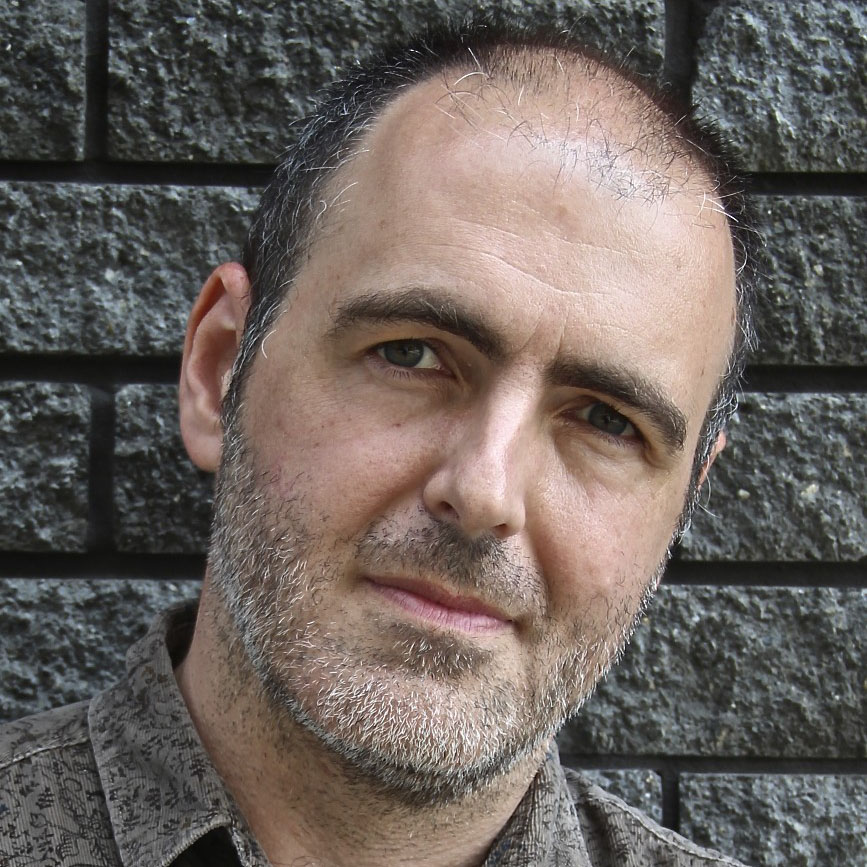
\includegraphics[width=5cm]{images/srp-mugshot} & 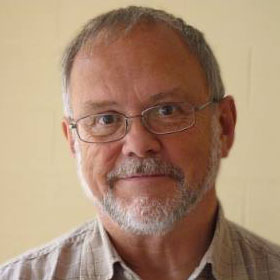
\includegraphics[width=5cm]{images/gdg-mugshot} \\
{\small steve.pettifer@manchester.ac.uk} & {\small graham.gough@manchester.ac.uk} \\
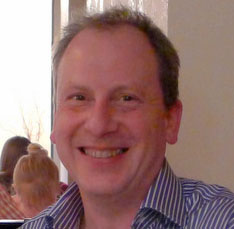
\includegraphics[width=5cm]{images/tljh-mugshot} & 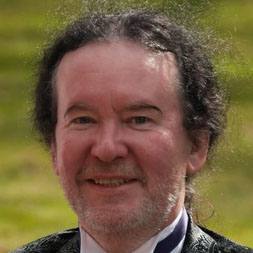
\includegraphics[width=5cm]{images/jtl-mugshot3.jpg} \\
{\small toby.howard@manchester.ac.uk}  & {\small john.latham@manchester.ac.uk} \\
\end{tabular}
\end{table}

\section{Acknowledgements}
These notes are largely our own work, but have been inspired in places by previous lab exercises created by Pete Jinks, John Sargeant and Ian Watson. We're very grateful to Alex Day, Alex Constantin, Hamza Mahmud and Ben Mulpeter for test driving and debugging the exercises.
